\documentclass[12pt]{zettel}

\renewcommand{\gregor}{\put(13.2,-3.0){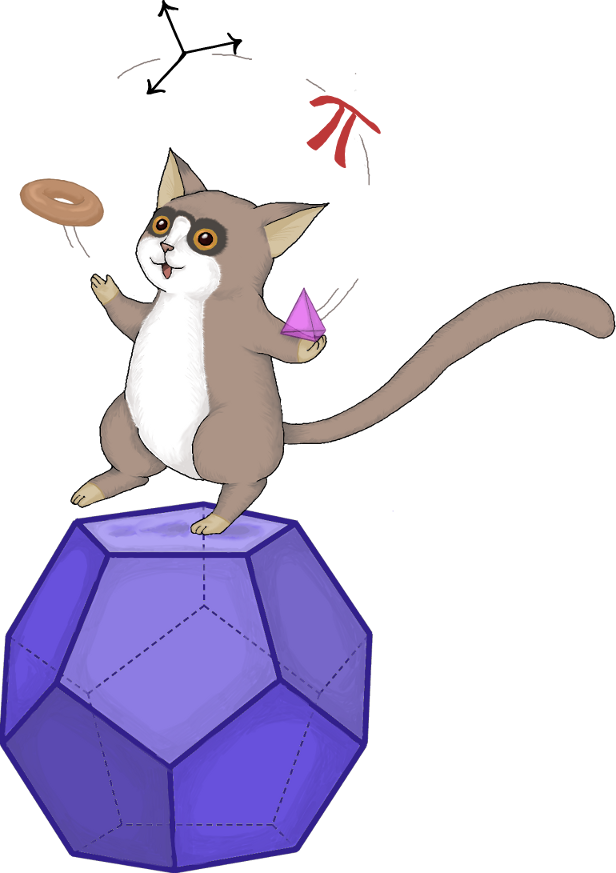
\includegraphics[scale=0.18]{cover}}}

\usepackage{framed}
\definecolor{shadecolor}{rgb}{.97,.97,.97}

\begin{document}

\renewcommand{\betreff}{}

\makeletterhead{}

\vspace{-2em}

\begin{center}
  \Large\textbf{\textsf{Bewerbung um den Witty-Förderpreis 2014: \\
  Matheschülerzirkel Augsburg }}
\end{center}

Aus der Anforderungsbeschreibung: "`Das Projekt soll
Kindern/Jugendlichen Selbstwertgefühl vermitteln, sie fördern und nachhaltig
Hilfe zur Selbsthilfe bieten."'

\begin{itemize}
\item Information über Verein und Aktivitäten inkl. evtl. Presseberichte
\item Wie setzen sich die rd. 50 TeilnehmerInnen am Mathematikcamp zusammen? Kann
man sich einfach bewerben - läuft es über Lehrer bzw. Schulen?
\item Wie sieht es mit der "`Nachhaltigkeit"' aus? d.h. wie geht es weiter, wenn
einzelne Schüler richtig +Feuer fangen und Begabung zeigen?
\item Wie lauten Ihre Ziele bei diesen Aktivitäten und Projekten? Gibt es zu
wenig Mathematikstudenten und setzen Sie deshalb bereits so früh an?
\item Das Preisgeld beträgt 10.000 Euro. Für das Camp benötigen Sie 7000,--. Wie
würden Sie das restliche Preisgeld sinnvoll verwenden?
\end{itemize}

\section{Bewerber}

Wir sind Doktoranden und Mitarbeiter des Instituts für Mathematik der
Universität Augsburg.

Kurzvorstellung

Zielsetzung


\section{Projektbeschreibung}

Wofür soll das Preisgeld eingesetzt werden?

Was macht das Projekt einmalig/einzigartig für unsere Region?


\section{Vision}

Was soll mit dem Projekt bewirkt werden?


\section{Zielgruppe(n)}

Wer lässt sich durch das Projekt erreichen?

Welchen Anspruch hat es?


\section{Budget}

Wofür wird das Preisgeld ausgegeben?
(grobe Aufschlüsselung nach Kostenarten)


\section{Öffentlichkeitsarbeit}

Wie wird die Öffentlichkeit über das Projekt informiert?
(Presse- und Öffentlichkeitsarbeit, Homepage,
Veranstaltungen etc.)


\section{Zeitrahmen}

Projektstart und voraussichtliche Dauer?

Sind
Verlängerungen
eingeplant?


\section{Ansprechpartner}
Für das
Projekt, bei
der
Durchführung


\section{Erfolgskontrolle}
Wie kann der
Erfolg
gemessen
werden?

\end{document}
